\chapter{Brugervejledning}

I dette kapitel gennemgåes brugen af det udviklede reservationssystem, Bookie. Vejledningen vil undervejs blive understøttet af billeder, der har til formål af eksemplificere de tilhørende instruktioner.

\section{Forestillinger}

Når Bookie åbnes, vises fanen \textit{Forestillinger}, der indeholder listen af forestillinger samt reservationsskærmen som set på figur \ref{screenshot:bookie}. På denne figur ses ydermere følgende elementer: Placeringen af lærredet i biografsalen, legenden over sædestatus (ledig, valgt, reserveret, og købt), samt formularen til reservation af sæder. En biografsal er imidlertid endnu ikke synlig, da der ikke er valgt en forestilling.

\begin{figure}[h]
  \centering
  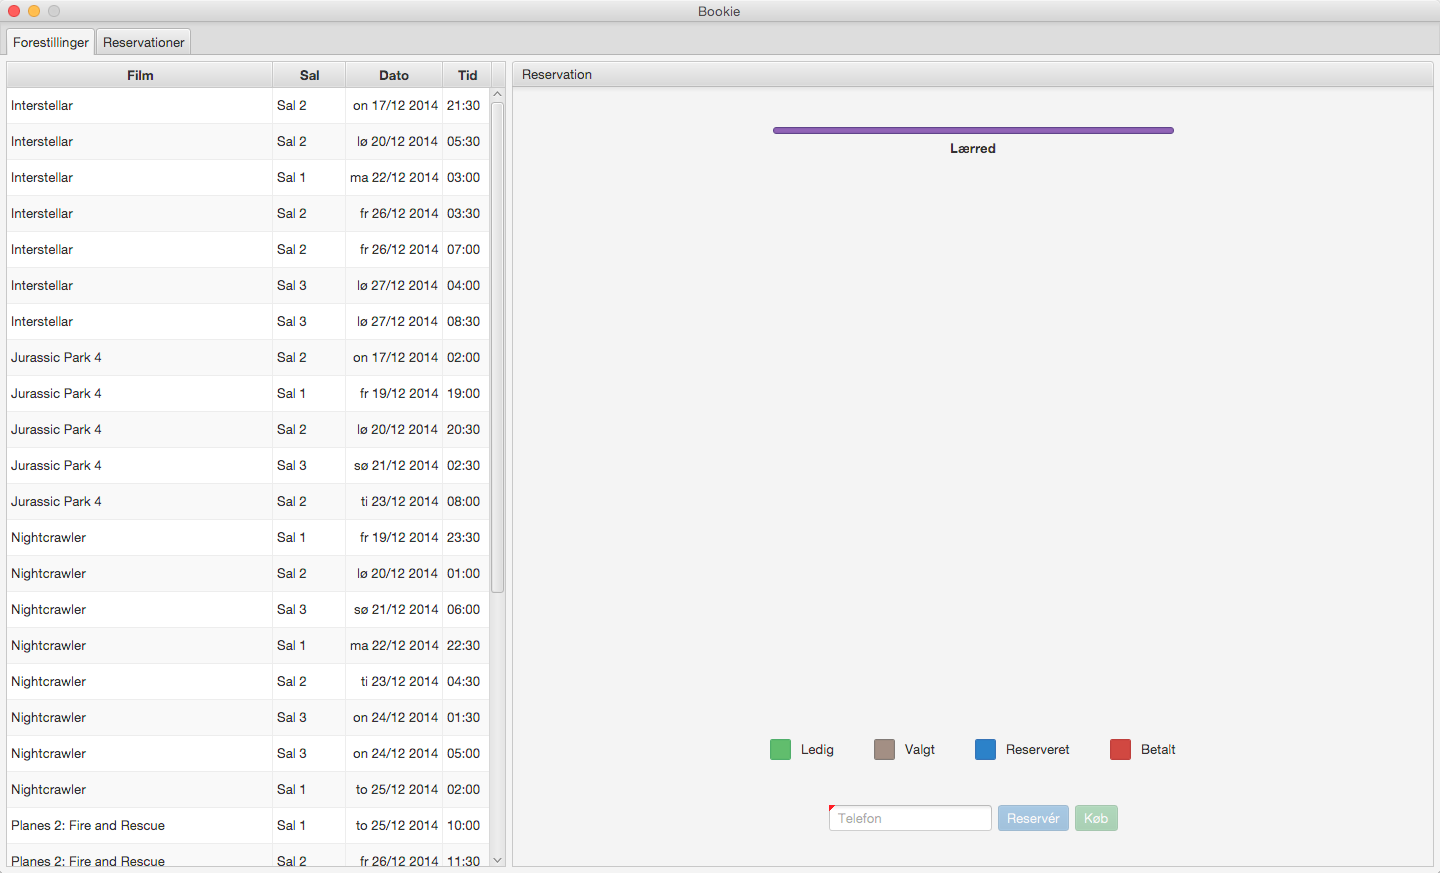
\includegraphics[width=\textwidth]{showtimes.png}
  \caption{Bookies startside straks efter opstart}
  \label{screenshot:bookie}
\end{figure}

\subsection{Valg af forestilling}

Der er mulighed for at sortere listen af forestillinger efter film, sal, dato, og tidspunkt. Det er derfor let at finde præcist den forestilling, som kunden måtte ønske. En forestilling vælges ved at klikke på den i listen.

%I tilfælde af, at listen med forestillinger bliver uoverskueligt lang, kan filtrering på enten film eller dato foretages således, at kun et ønsket udsnit af forestillinger er synlige på listen.

\begin{figure}[h]
  \centering
  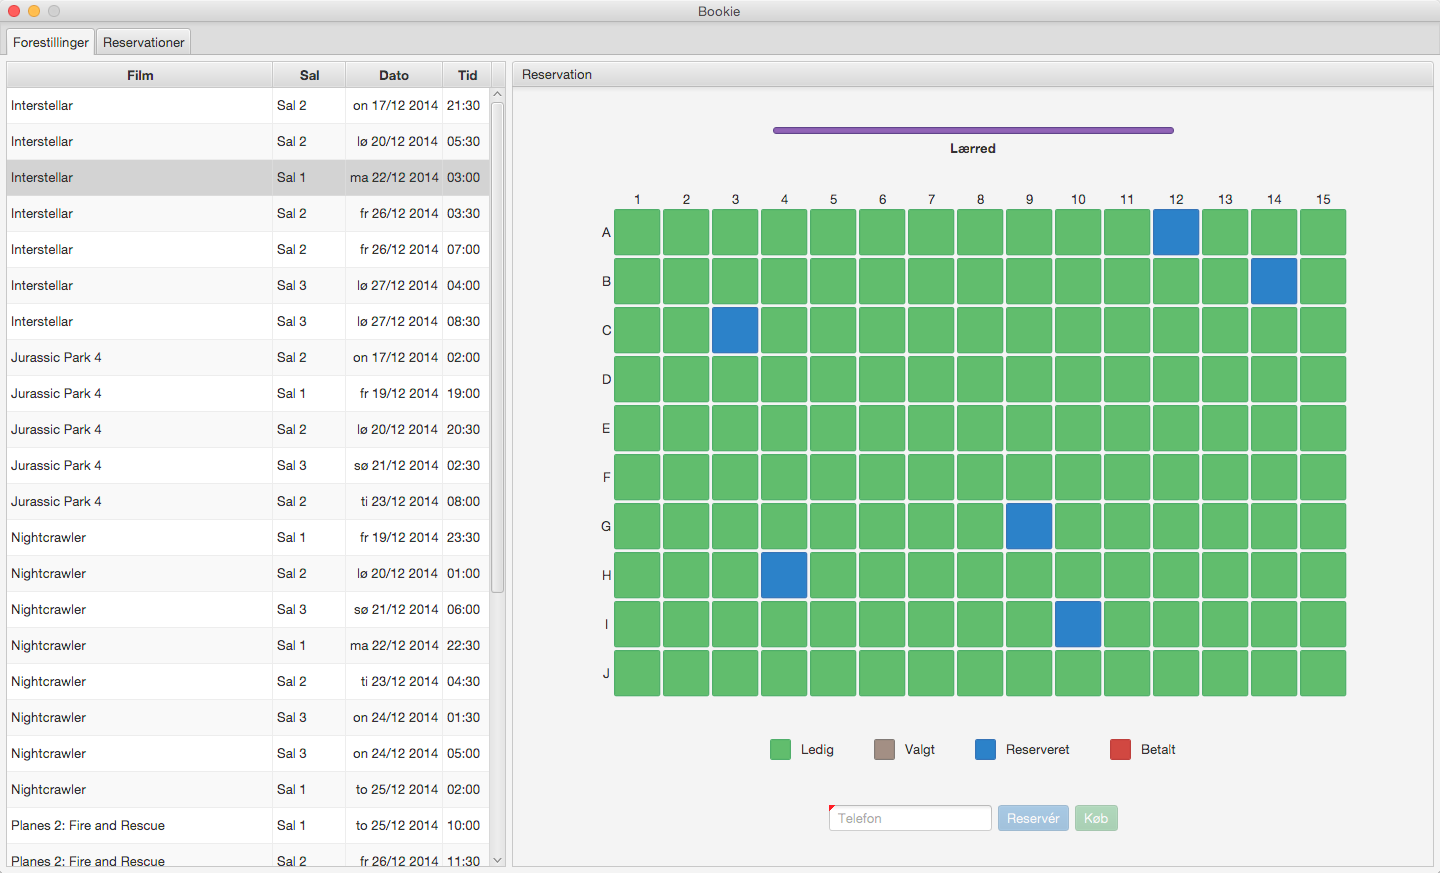
\includegraphics[width=\textwidth]{chosen-showtime.png}
  \caption{Udseende af biografsalen efter valg af forestilling}
  \label{screenshot:chosen-showtime}
\end{figure}

\subsection{Valg af sæder}

\begin{wrapfigure}[4]{r}{0.4\textwidth}
  \centering
  \vspace{-12pt}
  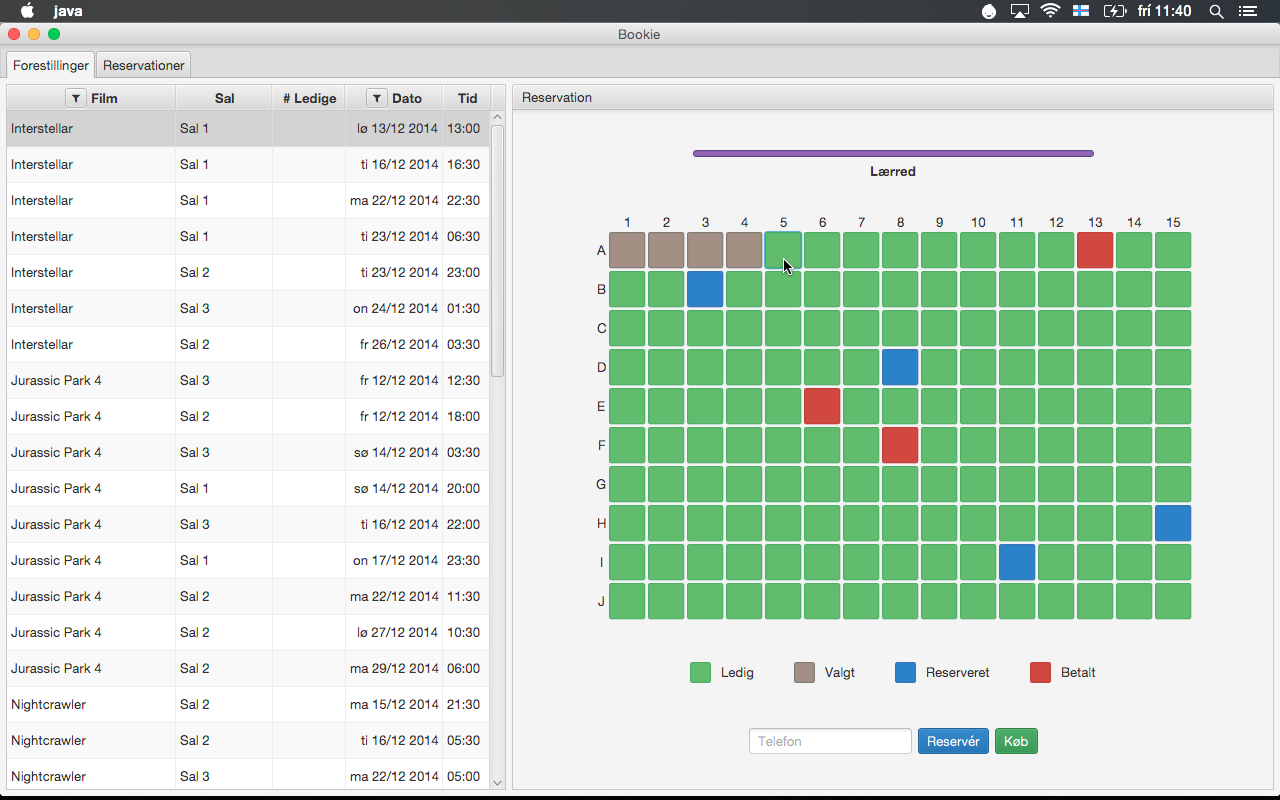
\includegraphics[width=0.35\textwidth]{chosen-seats.png}
  \caption{Eksempel på valg af sæder}
  \label{screenshot:chosen-seats}
\end{wrapfigure}

Holdes musen hen over et af de ledige sæder (markerede med grøn) og trykkes der på det, vil sædet skifte farve til grå som indikation på, at det er valgt til reservation.

Det er ikke muligt at oprette en reservation uden minimum at vælge et enkelt sæde.

\subsection{Reservation af sæder}

Efter de ønskede sæder er blevet valgt, er det muligt at indtaste et telefonnummer (se figur \ref{screenshot:phone-number}) for reservationen. Trykkes der derefter på \textit{Reservér}-knappen, ændres sædernes farve til blå som indikation på, at reservationen er gennemført. Det samme gør gældende med \textit{Køb-knappen}, hvor sædernes farve dog istedet vil ændres til rød. Efter gennemført reservation vil telefonnummer-feltet blive ryddet.

\begin{figure}[h]
  \centering
  \begin{minipage}[b]{0.4\linewidth}
    \centering
    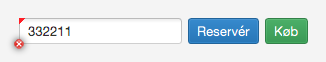
\includegraphics[width=\textwidth]{phone-number-invalid.png}
  \end{minipage}
  \hspace{0.5cm}
  \begin{minipage}[b]{0.4\linewidth}
    \centering
    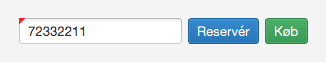
\includegraphics[width=\textwidth]{phone-number.png}
  \end{minipage}

  \caption{Eksempel på indtastning af ugyldigt (tv.) og gyldigt (th.) telefonnummer}
  \label{screenshot:phone-number}
\end{figure}

\section{Reservationer}

Når en reservation er oprettet, kan denne findes under fanen \textit{Reservationer}. Alle eksisterende reservationer kan ligeledes findes under denne fane som set på figur \ref{screenshot:all-reservations}.

\begin{figure}[h]
  \centering
  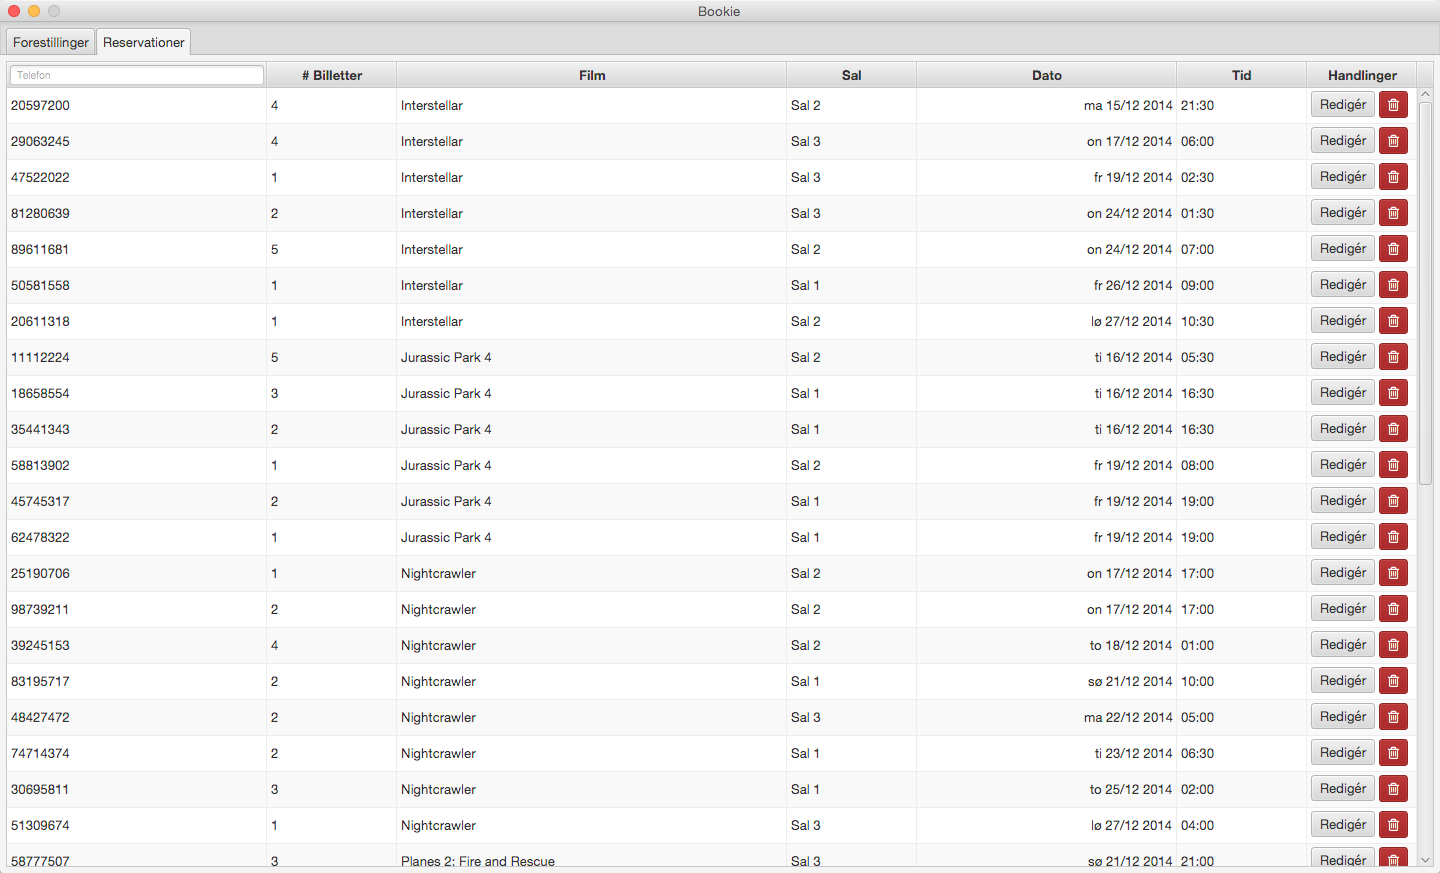
\includegraphics[width=\textwidth]{reservations.png}
  \caption{Visning af alle reservationer}
  \label{screenshot:all-reservations}
\end{figure}

\subsection{Filtrering af telefonnumre}

\begin{wrapfigure}[3]{r}{0.4\textwidth}
  \centering
  \vspace{-12pt}
  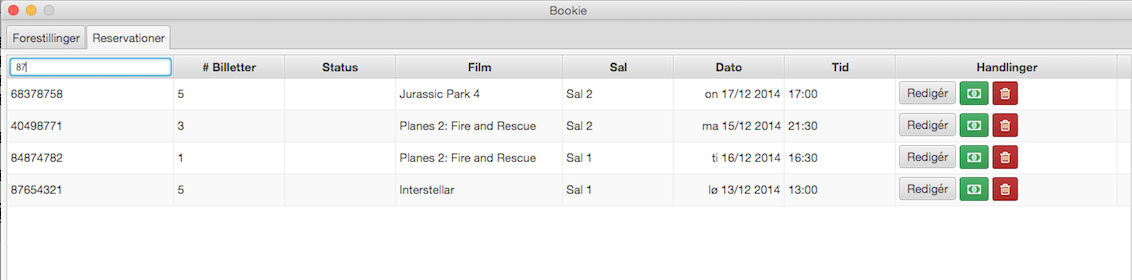
\includegraphics[width=0.35\textwidth]{filter3.png}
  \caption{Filtrering af telefonnumre}
  \label{screenshot:filter3}
\end{wrapfigure}

I øverste, venstre hjørne af reservationslisten findes et felt til filtrering af telefonnumrene (figur \ref{screenshot:filter3}). Der kan søges på enten fulde telefonnumre eller brydstykker af disse, hvilket gør det let af finde den eller de ønskede reservationer.

\subsection{Redigering af reservationer}

\begin{wrapfigure}{r}{0.4\textwidth}
  \centering
  \vspace{-12pt}
  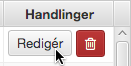
\includegraphics[width=0.2\textwidth]{edit-button.png}
  \caption{Mulighed for redigering af reservationer}
  \label{screenshot:edit-button}
\end{wrapfigure}

Når den ønskede reservation er fundet, kan denne hurtigt redigeres ved at trykke på \textit{Redigér}-knappen fundet i højre side af skærmen (figur \ref{screenshot:edit-button}). \textit{Forestillinger}-fanen vil da blive vist, hvorefter der enten kan fjernes sæder fra eller føjes flere sæder til den pågældende reservation (figur \ref{screenshot:edit-button}).

Skulle det ske, at reservationen ønskes flyttet til en anden forestilling, skal reservationen da først slettes, hvorefter en ny reservation kan oprettes til den ønskede forestilling. Sletning af reservationer gennemgåes nedenfor.

\subsection{Sletning af reservationer}

\begin{wrapfigure}{r}{0.4\textwidth}
  \centering
  \vspace{-12pt}
  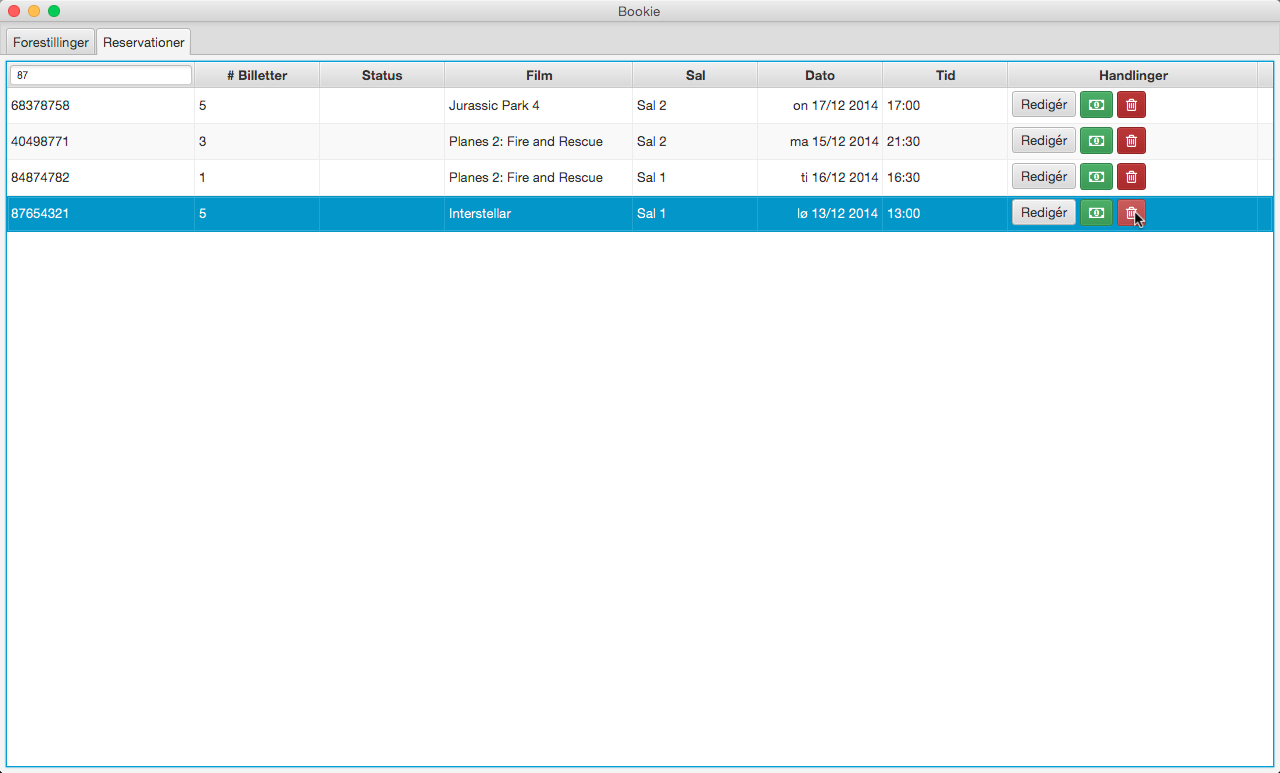
\includegraphics[width=0.2\textwidth]{delete-button.png}
  \caption{Mulighed for sletning af reservationer}
  \label{screenshot:delete-button}
\end{wrapfigure}

At slette er reservation er lige så smertefrit som at arbejde i resten af Bookie. Bliver der trykket på den røde knap med skraldespand-ikonet ved siden af \textit{redigér} knappen (som ses på \ref{screenshot:delete-button}, så kommer et pop-up (figur \ref{screenshot:delete-reservation}, hvor man kan vælge mellem \textit{cancel} eller \textit{ok}. Vælger ekspedienten \textit{cancel}, sker der ikke noget andet end, at pop-up'et forsvinder og \textit{Reservationer} forbliver som før. Vælger ekspedienten \textit{ok}, forsvinder den valgte reservation fra listen (figur \ref{screenshot:after-delete}).

\begin{figure} [h]
  \centering
  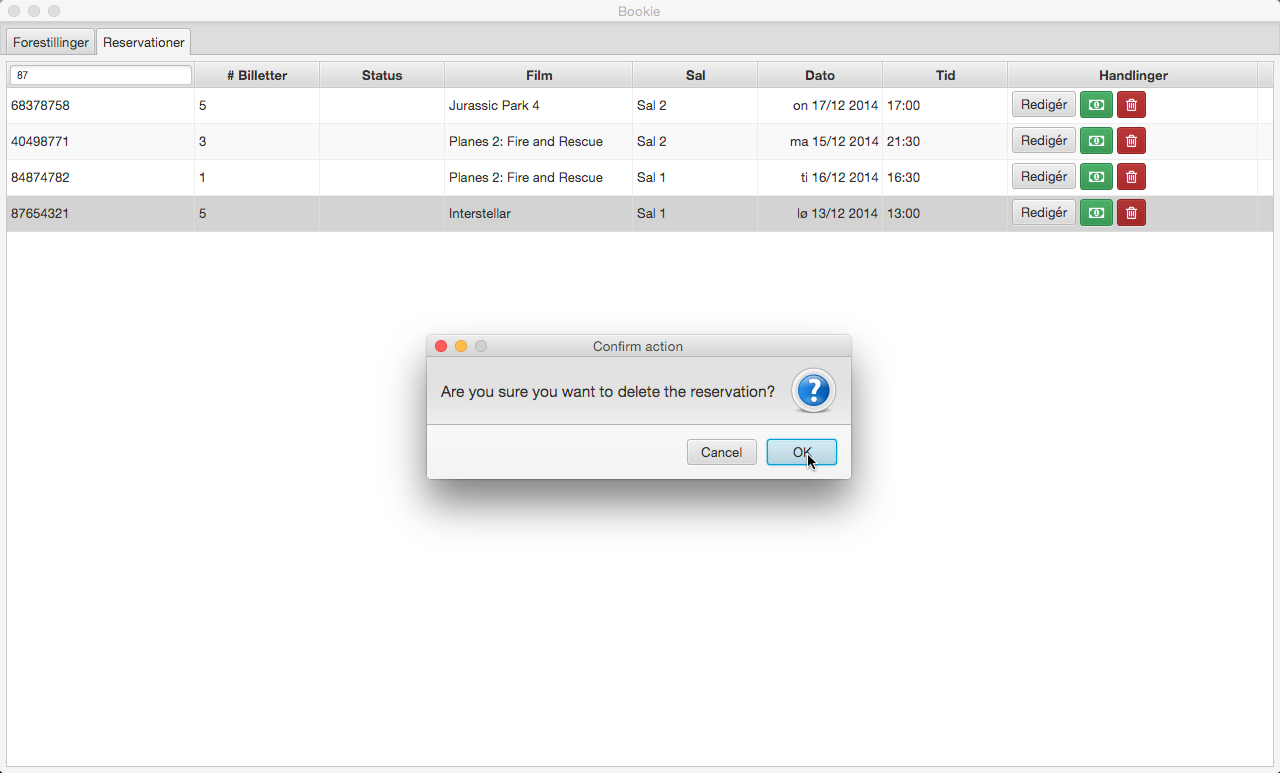
\includegraphics[width=0.4\textwidth]{delete-reservation.png}
  \caption{Sletning af reservation.}
  \label{screenshot:delete-reservation}
\end{figure}